% ============================================================
%  한국콘텐츠학회 논문지 투고용 심사 원고
%  ※ 심사 단계: 저자 정보 미기재
%  컴파일: xelatex main.tex (2회) + bibtex main + xelatex (2회)
%  또는: pdflatex 환경에서 kotex 사용 가능 시 pdflatex
% ============================================================
\documentclass[10pt,a4paper,twocolumn]{article}

% ── 한글 지원 ─────────────────────────────────────────────
\usepackage{kotex}

% ── 기본 패키지 ───────────────────────────────────────────
\usepackage{amsmath,amssymb}
\usepackage{booktabs}
\usepackage{graphicx}
\usepackage{array}
\usepackage{multirow}
\usepackage{xcolor}
\usepackage{tikz}
\usetikzlibrary{arrows.meta,shapes.geometric,positioning,fit,calc}
\usepackage[hidelinks]{hyperref}
\usepackage{caption}
\usepackage{enumerate}
\usepackage{setspace}
\usepackage{makecell}

% ── 페이지 레이아웃 ────────────────────────────────────────
\usepackage{geometry}
\geometry{
  a4paper,
  top=25mm, bottom=25mm,
  left=20mm, right=20mm,
  columnsep=6mm,
}

% ── 제목/캡션 스타일 ───────────────────────────────────────
\captionsetup{font=small, labelfont=bf, labelsep=period}
\captionsetup[table]{skip=3pt, position=top}
\renewcommand{\arraystretch}{1.10}
\setlength{\tabcolsep}{4pt}
\setlength{\emergencystretch}{2em}

% ── 그림 경로 ──────────────────────────────────────────────
\graphicspath{{figures/}}

% ── 참고문헌 스타일 ────────────────────────────────────────
\usepackage[numbers,sort&compress]{natbib}
\bibliographystyle{unsrt}

% ── 두 컬럼 제목 블록용 매크로 ────────────────────────────
\makeatletter
\newcommand{\koabstract}[1]{%
  \small\textbf{요약:~}#1\par}
\newcommand{\enabstract}[1]{%
  \small\textbf{Abstract:~}#1\par}
\makeatother

% ============================================================
\begin{document}

% ── 제목 (두 컬럼에 걸침) ────────────────────────────────
\twocolumn[{%
\begin{center}
{\fontsize{14}{17}\bfseries
TA-BRPL: 저전력 손실 네트워크에서 Sinkhole 경로 장악 완화를 위한\\
신뢰 기반 Backpressure RPL\par}
\vspace{4pt}
{\fontsize{11}{14}\bfseries
TA-BRPL: Trust-Aware Backpressure RPL for Mitigating\\
Sinkhole-Induced Route Capture in Low-Power and Lossy Networks\par}
\vspace{6pt}
% 저자 정보 (심사 단계 제외)
{\small 저자 정보는 심사 후 기재\par}
\vspace{8pt}
\hrule\vspace{6pt}

% 국문 초록
\begin{minipage}{0.96\textwidth}
\koabstract{%
저전력 손실 네트워크(LLN)에서 RPL은 낮은 제어 오버헤드와 토폴로지 안정성을 중시하므로,
한 번 선택된 부모 노드가 오래 유지되는 경향이 있다.
이 특성은 sinkhole 공격자가 낮은 rank를 허위로 광고해 경로를 유인할 때
장기적인 \emph{경로 장악(route capture)}으로 이어질 수 있다.
공격자는 먼저 트래픽을 자신에게 집중시키고,
이후 선택적 포워딩(selective forwarding)으로 가용성을 저하시킨다.
PDR은 드롭 이후 피해를 반영하지만, 드롭 이전의 경로 장악 단계를 직접 측정하지 못한다.
반대로 신뢰 하락을 즉시 퇴출로 연결하면 부모 교체(churn)가 폭증해
보안과 안정성 사이의 trade-off가 악화된다.
또한 BRPL류의 queue-aware 라우팅은 혼잡 우회에는 강하지만,
공격자가 큐 광고를 조작하거나 초기에는 정상 포워딩으로 신뢰를 위장하는 경우
공격자가 선호 부모 위치를 장기간 유지할 위험이 있다.
본 논문은 Backpressure RPL(BRPL)의 부모 선택 점수에
경량 신뢰 패널티를 직접 결합한 \textbf{TA-BRPL}을 제안한다.
TA-BRPL은 (i)~전달 신뢰도($T_{fwd}$), (ii)~제어 평면 일관성($T_{ctrl}$),
(iii)~큐 정직성($T_{hon}$)을 가중 기하 평균으로 집계한 신뢰값을
BRPL 부모 선택 비용에 소프트 패널티로 반영한다.
또한 비대칭 EWMA, 2단계 review/blacklist, admission/dwell/switch-margin 정책으로
신뢰를 \emph{탐지 알람}이 아닌 \emph{라우팅 의사결정}에 안정적으로 통합한다.
Contiki-NG/Cooja에서 밀도별 층화 랜덤 토폴로지 75개와
토폴로지당 5개 MAC 시드(총 750회)를 사용한 쌍체 실험 결과,
TA-BRPL은 BRPL 대비 공격자 경유율(att\_share)을
평균 $\Delta = -0.0169$ ($p < 10^{-4}$, 승률 76\%) 감소시키고,
hit\_ratio를 $\Delta = -0.0166$ 낮추며,
공격 구간 PDR을 $\Delta = +0.0102$ ($p = 0.002$) 개선한다.
churn 증가는 $\Delta = +0.0364$로 제한되며
사전 선언한 실무 상한 $+0.1$의 범위 안에 머문다.
이 결과는 LLN 보안에서 핵심 과제가 ``더 민감한 탐지''만이 아니라,
신뢰를 라우팅 metric에 어떻게 결합하고 그로 인한 불안정을 어떻게 제어하느냐에 있음을 보여준다.}
\vspace{4pt}

\noindent\textbf{핵심어:}
LLN, RPL, BRPL, Sinkhole 공격, 신뢰 기반 라우팅, 경로 장악, 선택적 포워딩, Contiki-NG
\end{minipage}

\vspace{6pt}

% 영문 초록
\begin{minipage}{0.96\textwidth}
\enabstract{%
In low-power and lossy networks (LLNs), RPL prioritizes low control overhead and topology
stability, causing selected parent nodes to persist for extended periods.
This property becomes a vulnerability under sinkhole attacks:
an attacker forges an attractive low-rank advertisement to induce
\emph{route capture}---concentrating upstream traffic through itself---and subsequently
drops packets selectively to degrade availability.
PDR-centric evaluation misses this early capture phase, since packet loss only manifests later.
Conversely, aggressively evicting distrusted parents triggers churn explosion.
Queue-aware protocols such as Backpressure RPL (BRPL) improve congestion handling,
yet remain exploitable when an attacker manipulates queue advertisements or behaves benignly
long enough to retain parent preference.
We propose \textbf{TA-BRPL}, a trust-aware extension that embeds a lightweight trust penalty
directly into the BRPL parent-selection score.
TA-BRPL aggregates three trust signals---(i)~forwarding fidelity ($T_{fwd}$),
(ii)~control-plane consistency ($T_{ctrl}$), and (iii)~queue-advertisement honesty ($T_{hon}$)---%
via a weighted geometric mean, and couples the result to routing
through asymmetric EWMA, two-stage review/blacklist validation, and stabilization gates
(admission threshold, dwell time, and switch margin).
Experiments across 75 stratified random topologies with five MAC seeds each
(750 simulations) in Contiki-NG/Cooja show that TA-BRPL reduces attacker traffic share
by $\Delta = -0.0169$ ($p < 10^{-4}$, 76\% win-rate) and hit ratio by $\Delta = -0.0166$,
improves attack-phase PDR by $\Delta = +0.0102$ ($p = 0.002$),
and limits churn to $\Delta = +0.0364$, well within the pre-declared bound of $+0.1$.
These results suggest that the central challenge in LLN secure routing is not only detecting
malicious parents, but integrating trust into routing decisions without sacrificing stability.}
\vspace{4pt}

\noindent\textbf{Keywords:}
LLN, RPL, BRPL, sinkhole attack, trust-aware routing, route capture,
selective forwarding, Contiki-NG
\end{minipage}

\vspace{8pt}\hrule\vspace{10pt}
\end{center}
}]  % end twocolumn title block


% ============================================================
\section{서론}
\label{sec:intro}

저전력 손실 네트워크(LLN)는 스마트 빌딩, 산업 모니터링, 정밀 농업처럼
배터리 제약과 링크 손실이 큰 환경에서 데이터를 수집한다.
이 환경의 라우팅 프로토콜은 단순한 최단 경로 최적화보다
안정성, 제어 오버헤드, 재전송 비용, 경로 복원력을 함께 고려해야 한다.
IETF 표준 RPL~\cite{rfc6550}은 Trickle~\cite{rfc6206} 기반 DIO로 DODAG를 구성하고,
MRHOF~\cite{rfc6719}, OF0~\cite{rfc6552} 같은 목적함수로 부모를 선택한다.
특히 MRHOF는 히스테리시스를 통해 빈번한 부모 교체(churn)를 억제하도록 설계되어 있으나,
이러한 안정성 지향 정책은 한 번 잘못 선택한 부모를 오래 유지하게 만들어
보안 측면에서는 새로운 취약점이 될 수 있다~\cite{rfc6551,rpl_stability2015}.

즉 LLN 보안의 핵심은 \textbf{보안-안정성 trade-off}다.
악성 부모를 빨리 배제하면 route capture를 줄일 수 있지만,
동적 신뢰 신호를 너무 공격적으로 반영하면 라우팅이 진동하고
네트워크 전체 churn이 증가한다.
반대로 부모 전환을 지나치게 보수적으로 억제하면 평상시 안정성은 좋아지지만,
sinkhole 공격자는 오랫동안 preferred parent로 남아
하위 트리의 트래픽을 집중시킬 수 있다.

이 부모 선택 메커니즘은 \textbf{sinkhole 공격}의 직접적인 표적이다.
공격자는 허위로 낮은 rank를 광고해 주변 노드를 유인하고,
초기에는 패킷을 정상 전달함으로써 겉보기 PDR을 유지한다.
그러나 그 사이 점점 더 많은 노드가 공격자를 경유하게 되며,
\emph{경로 장악(route capture)}이 완성되면
공격자는 selective forwarding으로
가용성을 크게 훼손할 수 있다.
Karlof와 Wagner~\cite{karlof2003}, RFC~7416~\cite{rfc7416},
Wallgren 등~\cite{secrpl}, Mayzaud 등~\cite{mayzaud2016}은
이러한 위협이 단순한 패킷 드롭이 아니라
유인$\rightarrow$장악$\rightarrow$드롭의 연쇄 구조를 가진다고 설명한다.
문제는 기존 평가가 주로 PDR에 집중해
실제 드롭이 발생하기 전의 장악 단계를 놓친다는 점이다.

기존 방어는 대체로 세 계열로 정리된다.
\emph{인증 기반 secure routing}은 rank 조작을 암호학적으로 차단하지만,
공개키 인프라와 서명 검증 비용이 제한된 센서 네트워크에 부담이 크다~\cite{dvir2011,roll_trust}.
\emph{IDS 기반 이상 탐지}는 비정상 경로를 식별하지만,
중앙 모니터 의존성 또는 탐지-라우팅 분리 문제가 남는다~\cite{raza2013,iotroute_survey2016}.
\emph{신뢰/평판 기반 라우팅}은 라우팅에 직접 반영한다는 점에서 더 적합하지만,
신뢰 하락을 즉각적인 전환으로 연결할 때
stability cost를 어떻게 제어할지 충분히 설명하지 않는 경우가 많다~\cite{sectrust2019,rftrust2021,pccrpl2022,trustmodel2022}.
실제로 본 연구의 초기 TA-BRPL 버전(v1)도 게이트 없이 신뢰를 강하게 반영했을 때
churn이 +2.43까지 폭증했다.

한편 BRPL~\cite{brpl}은 backpressure와 queue gradient를 이용해
혼잡 회피와 라우팅 적응성을 높인다는 점에서 유망한 LLN 확장형 RPL이다.
그러나 queue-aware라는 장점이 곧바로 보안 강건성을 의미하지는 않는다.
공격자가 낮은 rank와 낮은 queue를 함께 광고하거나,
초기에는 정상 포워딩으로 신뢰를 위장한 뒤 드롭을 시작하면,
BRPL의 queue term은 오히려 공격자를 선호 부모 위치에 오래 유지할 수 있다.
즉 BRPL류는 혼잡에 강하지만,
queue honesty와 control-plane manipulation을 별도로 다루지 않는 한
sinkhole 하에서 불완전하다.

본 논문은 다음 두 연구 질문에 답한다.
\textbf{RQ1:} sinkhole의 경로 장악 단계에서 PDR 저하 이전에 공격자 경유를 감소시킬 수 있는가?
(지표: att\_share, hit\_ratio)
\textbf{RQ2:} 신뢰를 라우팅 metric에 결합할 때 churn 폭증을 구조적으로 제어하면서도 방어 효과를 유지할 수 있는가?
(지표: churn $\Delta \leq +0.1$, PDR 비열세)
이를 위해 H1(격리 개선), H2(PDR 비열세), H3(안정성 상한)을 사전 선언하고,
경로 장악 억제를 1차 목표로 하는 평가 프레임을 채택한다.

본 논문의 기여는 네 가지다.
\textbf{C1}: 방어 1차 목표를 PDR이 아닌 경로 장악 억제(att\_share, hit\_ratio)로 재정의한다.
\textbf{C2}: BRPL metric에 전달 신뢰도($T_{fwd}$), 제어 평면 일관성($T_{ctrl}$),
큐 정직성($T_{hon}$)을 소프트 패널티로 직접 통합한다.
\textbf{C3}: 비대칭 EWMA, review/blacklist, admission/dwell/switch-margin을 포함한
안정화 설계 원칙으로 trust-aware routing의 churn 문제를 구조적으로 다룬다.
\textbf{C4}: 밀도별 층화 랜덤 토폴로지 75개와 5개 MAC 시드를 사용한
쌍체 통계 검증으로 효과의 일관성과 경계 조건을 함께 제시한다.


% ============================================================
\section{관련 연구}
\label{sec:background}

\subsection{RPL, MRHOF, 그리고 LLN 안정성}

RPL~\cite{rfc6550}은 LLN에서 표준 IPv6 라우팅 계층으로 자리잡았고,
Trickle~\cite{rfc6206} 기반 DIO 전파와 목적함수 선택을 통해
DODAG를 유지한다.
MRHOF~\cite{rfc6719}는 ETX 중심 최적화와 히스테리시스를 결합해
부모 재선택의 진동을 줄이고, OF0~\cite{rfc6552}는 더 단순한 대안을 제공한다.
RFC~6551~\cite{rfc6551}은 경로 메트릭과 제약을 표준화하며,
동적 메트릭 결합 시 라우팅 불안정성이 생길 수 있음을 내포한다.
후속 연구와 survey들은 RPL에서 성능 저하의 상당 부분이
``어떤 메트릭을 쓸 것인가''보다 ``언제 부모를 바꿀 것인가''에 달려 있음을 보고했다~\cite{rpl_stability2015}.
즉 LLN 라우팅에서는 안정한 parent-selection policy가
성능과 보안 모두의 전제 조건이다.
이와 맞물려 update policy를 적응적으로 조절해
불필요한 churn을 줄이려는 연구도 이어졌다~\cite{ghaleb2018}.

\subsection{RPL 공격: sinkhole, blackhole, selective forwarding}

Karlof와 Wagner~\cite{karlof2003}는 무선 센서 네트워크에서
sinkhole과 selective forwarding을 기본 위협으로 정리했고,
RFC~7416~\cite{rfc7416}은 이를 RPL의 topology manipulation 위협으로 공식화했다.
Mayzaud 등~\cite{mayzaud2016}은 rank 위조, version 조작, sinkhole,
forwarding 공격을 포함한 taxonomy를 제시했으며,
Wallgren 등~\cite{secrpl}은 RPL 기반 IoT에서
``패킷 드롭이 시작된 뒤에야 탐지하는'' 평가 공백을 지적했다.
version-number attack의 실증 분석도 별도로 보고되었다~\cite{aris2016}.
최근 survey들도 동일한 문제를 반복한다~\cite{sinkhole_survey2023,rpl_survey2025,raoof2019}.
즉 많은 연구가 여전히 PDR 저하를 공격 효과의 중심 지표로 사용하지만,
실제로는 route capture가 먼저 형성되고,
그 뒤 selective forwarding이나 blackhole이 피해를 증폭시킨다.

\subsection{Trust-based routing, watchdog, IDS, secure routing}

watchdog와 reputation은 신뢰 기반 라우팅의 고전적 출발점이다.
Marti 등~\cite{marti2000}은 수동 도청으로 forwarding misbehavior를 포착하는
기본 아이디어를 제시했고,
Ganeriwal 계열의 연구~\cite{airtime_trust,rfsn2008}는 이를
센서 네트워크용 분산 평판 모델로 확장했다.

RPL 방어로 오면 접근은 세 갈래로 나뉜다.
첫째, \emph{secure routing / 인증 기반}은
VeRA~\cite{dvir2011}처럼 rank/version 조작을 암호학적으로 방지한다.
그러나 키 관리와 서명 검증 비용, 내부자 공격 취약성이 남는다.
둘째, \emph{IDS 기반}은 SVELTE~\cite{raza2013}처럼
경로 이상을 탐지하지만 중앙 모니터 또는 별도 제어 채널 의존성이 높고,
탐지 결과가 라우팅 metric에 직접 결합되지 않는 경우가 많다~\cite{iotroute_survey2016}.
셋째, \emph{trust-aware routing}은
SecTrust-RPL~\cite{sectrust2019}, RFTrust~\cite{rftrust2021},
PCC-RPL~\cite{pccrpl2022}, Sensors 2022 계열~\cite{trustmodel2022,trustids2022}처럼
신뢰를 라우팅에 직접 반영한다.
이 흐름은 route capture 억제에 더 직접적이지만,
신뢰 하락을 곧바로 parent eviction으로 연결할 경우
오탐과 churn을 어떻게 다룰지에 대한 정책 설명은 상대적으로 약하다.

\subsection{BRPL, backpressure, queue-aware routing}

Tassiulas와 Ephremides~\cite{tassiulas1992}의 역압 이론과
BCP~\cite{bcp2010}는 큐 gradient를 사용한 다중 홉 수집 경로의
안정성과 적응성을 보여주었다.
BRPL~\cite{brpl}은 이 아이디어를 RPL 위에 올려
rank, ETX, queue 차이를 함께 고려한다:
\begin{equation}
  S_{\text{BRPL}}(v) = w_p\!\cdot\!\text{rank}(v)
                     + w_q\!\cdot\!\Delta Q(v)
                     + w_l\!\cdot\!\text{ETX}(v).
  \label{eq:brpl}
\end{equation}
이 방식은 혼잡 회피와 부하 분산에서는 강점을 갖지만,
보안적으로는 queue advertisement의 정직성을 전제한다.
공격자가 낮은 rank와 낮은 queue를 함께 광고하면,
queue-aware metric은 공격자를 더 매력적인 부모로 만들 수 있다.
즉 BRPL은 혼잡에는 강하지만 sinkhole에는 충분조건이 아니다.

\subsection{Routing stability, hysteresis, churn}

신뢰 기반 라우팅의 어려움은 탐지보다도 안정성이다.
MRHOF의 히스테리시스는 본래 링크 품질 요동을 완화하기 위한 장치였지만~\cite{rfc6719},
동적 신뢰 신호가 들어오면 그 자체가 새로운 진동 원인이 된다.
따라서 trust-aware routing에서 핵심 질문은
``누가 악성인가''만이 아니라 ``얼마나 빨리, 어떤 증거에서, 어떤 비용으로
부모를 바꿀 것인가''다.
본 연구는 이 stability 축을
Related Work의 핵심 비교 기준으로 전면에 둔다.

\subsection{비교표와 연구 갭}

표~\ref{tab:relwork}은 관련 연구를
``라우팅 직접 반영 여부'', ``중앙 의존성'', ``queue honesty 반영 여부'',
``명시적 churn 제어 여부''의 네 축으로 비교한다.
기존 연구는 한 축에서는 강점을 보이지만,
queue-aware BRPL의 보안 공백과
trust-aware routing의 stability cost를 동시에 다루는 설계는 드물다.

\begin{table*}[!t]
\centering\small
\caption{RPL 보안 방어 계열 비교 (O: 충족, P: 부분, X: 미충족)}
\label{tab:relwork}
\resizebox{\linewidth}{!}{%
\setlength{\tabcolsep}{3.5pt}
\begin{tabular}{lllccccl}
\toprule
계열 & 대표 연구 & 핵심 아이디어 &
\makecell{라우팅\\직접 반영} & \makecell{중앙\\의존} & \makecell{Queue\\honesty} & \makecell{Churn\\제어} & 주요 한계 \\
\midrule
인증/서명  & VeRA \cite{dvir2011}             & DIO 서명 검증           & $\times$ & $\times$ & $\times$ & $\times$ & PKI 비용, 내부자 취약 \\
IDS 기반   & SVELTE \cite{raza2013}           & 런타임 이상 탐지        & $\times$ & $\circ$  & $\times$ & $\times$ & 중앙 모니터, 라우팅 미반영 \\
신뢰/평판  & SecTrust-RPL \cite{sectrust2019} & watchdog$\to$라우팅     & $\circ$  & $\times$ & $\times$ & $\triangle$ & churn 위험, gate 설계 약함 \\
신뢰/탐지  & RFTrust \cite{rftrust2021}       & ML 탐지+차단            & $\triangle$ & $\triangle$ & $\times$ & $\times$ & 탐지-라우팅 분리, stability 미검증 \\
역압 기반  & BRPL \cite{brpl}                 & 큐 기울기 경로 선택     & $\circ$  & $\times$ & $\times$ & $\circ$  & 큐 광고 신뢰 전제(조작 취약) \\
\midrule
\textbf{본 연구} & \textbf{TA-BRPL}           & \textbf{3축 trust + BRPL coupling + gate} & $\circ$ & $\times$ & $\circ$ & \textbf{$\circ$(명시)} & 단일 공격자·UDGM \\
\bottomrule
\end{tabular}%
}
\end{table*}

\noindent
표~\ref{tab:relwork}에서 보듯,
인증 기반은 route capture를 원천 차단하지만 비용이 크고,
IDS 기반은 탐지력은 있으나 라우팅과 분리되어 있으며,
신뢰 기반은 직접 반영의 장점이 있지만 stability policy가 약하다.
BRPL은 혼잡과 queue imbalance에는 강하나
queue honesty와 control-plane lure를 검증하지 않는다.
따라서 본 연구의 핵심 연구 갭은
\emph{``queue-aware LLN routing에 trust를 직접 결합하되,
그로 인한 churn을 명시적 게이트로 제어하는 설계''}로 정리된다.


% ============================================================
\section{시스템 및 위협 모델}
\label{sec:threat}

본 절은 TA-BRPL이 해결하려는 문제를
네트워크 구조, 공격자 능력, 공격 목표의 관점에서 구체화한다.
핵심은 sinkhole을 단순 packet drop이 아니라
\emph{경로 장악을 먼저 만들고 이후 드롭을 실행하는 2단계 공격}으로 보는 것이다.

\begin{figure}[t]
\centering
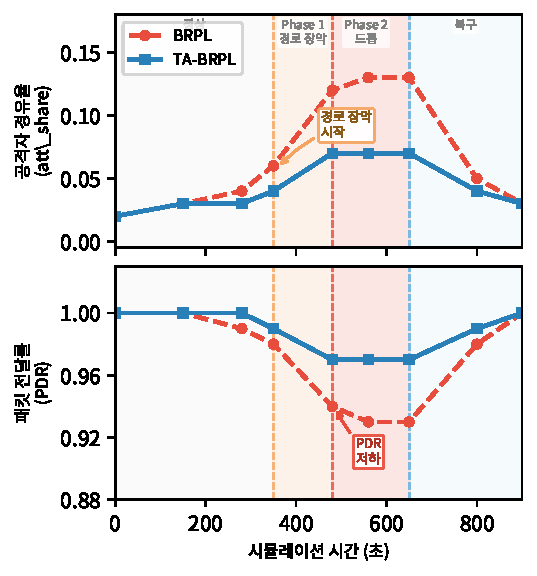
\includegraphics[width=\columnwidth]{fig_jkcs_threat.pdf}
\caption{Sinkhole 2단계 공격 개념 타임라인.
  Phase~1에서 공격자는 낮은 rank와 매력적인 queue 상태를 광고해
  att\_share를 먼저 상승시키고(route capture),
  Phase~2에서 selective forwarding을 시작해 PDR을 저하시킨다.
  TA-BRPL의 1차 목표는 Phase~1을 조기에 억제하는 것이다.}
\label{fig:threat}
\end{figure}

\subsection{네트워크 구조}

대상 네트워크는 하나의 루트(sink)와 다수의 배터리 기반 센서 노드로 구성된
다중 홉 LLN이다.
각 노드는 주기적으로 UDP 데이터를 생성해 루트로 전송하고,
상향 경로는 preferred parent 선택에 의해 결정된다.
이 구조에서는 특정 노드가 많은 자식의 parent가 되는 순간
하위 트리 전체의 트래픽이 그 노드를 통과하게 되므로,
route capture는 단일 링크 문제가 아니라 서브트리 단위의 구조 문제다.

\subsection{공격자 능력과 제한}

공격자는 네트워크에 합법적으로 참여한 단일 내부자 노드로 가정한다.
공격자는 다음을 수행할 수 있다.
\begin{itemize}
\item 실제보다 낮은 rank를 광고해 부모 선택을 왜곡한다.
\item 자신을 경유하는 상향 데이터 패킷의 일부 또는 전부를 드롭한다.
\item 초기에는 정상 전달을 유지해 의심을 늦춘다.
\item BRPL류에서 불리하지 않은 queue 상태를 광고한다.
\end{itemize}
반대로 본 논문은 다중 공모 공격자, 물리 계층 jamming, ACK 위조,
암호학적 키 관리 파괴는 가정하지 않는다.

\subsection{공격 정의와 공격 시점}

\textbf{sinkhole}은 허위로 낮은 rank를 광고해 경로를 유인하는 단계다.
\textbf{blackhole}은 자신을 경유한 패킷을 전부 버리는 경우이며,
\textbf{selective forwarding}은 일정 비율만 드롭해
은닉성을 높이는 경우다.
본 실험은 이들을 분리된 세 공격이 아니라
``유인 이후 50\% selective drop''이라는 연속 시나리오로 사용한다.
즉 공격자는 먼저 route lure로 parent concentration을 유도하고,
충분히 장악된 뒤 드롭을 시작한다.

\subsection{공격 목적과 방어 목적}

공격자의 목적은 세 가지로 정리된다.
\begin{itemize}
\item \textbf{route capture}: 더 많은 노드가 공격자를 preferred parent로 채택하게 하기
\item \textbf{traffic lure}: 전체 상향 트래픽의 더 큰 비율을 공격자에게 집중시키기
\item \textbf{availability degradation}: 이후 drop으로 PDR을 낮추기
\end{itemize}

이에 대응해 TA-BRPL의 방어 목적도 세 층으로 둔다.
\begin{itemize}
\item \textbf{1차 목표}: att\_share와 hit\_ratio를 줄여 장악 강도와 오염 범위를 완화
\item \textbf{2차 목표}: 공격 구간 PDR을 비열세 범위 이상으로 유지
\item \textbf{3차 목표}: 방어 과정에서 증가하는 churn을 실무 상한 안으로 통제
\end{itemize}


% ============================================================
\section{제안 기법: TA-BRPL}
\label{sec:design}

\subsection{설계 철학: 소프트 패널티 + 보수적 게이트}

TA-BRPL은 두 설계 원칙에 따라 구성된다.
\textbf{P1 (소프트 페널티):} 불신 노드를 즉시 차단하는 대신,
신뢰 저하를 부모 선택 비용에 연속적으로 반영해 점진적으로 비선호 노드로 강등한다.
\textbf{P2 (보수적 전환):} 충분한 증거가 누적되기 전에는 부모를 교체하지 않으며,
admission/dwell/switch-margin 게이트가 이 원칙을 각각 다른 failure mode에서 시행한다.

그림~\ref{fig:arch}는 신뢰 파이프라인 전체 구조를 보여준다.
세 신호가 집계된 뒤 비대칭 EWMA로 업데이트되고,
BRPL 점수에 소프트 패널티로 반영된다.

\begin{figure}[t]
\centering
\resizebox{\columnwidth}{!}{%
\begin{tikzpicture}[
  node distance=0.4cm and 1.1cm,
  box/.style ={rectangle,draw,fill=blue!8,rounded corners=2pt,
               minimum width=26mm,minimum height=7mm,align=center,font=\scriptsize},
  sbox/.style={rectangle,draw,fill=orange!12,rounded corners=2pt,
               minimum width=26mm,minimum height=7mm,align=center,font=\scriptsize},
  agg/.style ={rectangle,draw,fill=green!12,rounded corners=2pt,
               minimum width=26mm,minimum height=9mm,align=center,font=\scriptsize},
  rbox/.style={rectangle,draw,fill=gray!10,rounded corners=2pt,
               minimum width=30mm,minimum height=13mm,align=center,font=\tiny},
  arrow/.style={-{Stealth[scale=0.7]},semithick},
]
\node[box]  (tf)                    {$T_{fwd}$: 전달 신뢰도};
\node[box,  below=of tf] (tc)       {$T_{ctrl}$: 제어 평면};
\node[box,  below=of tc] (th)       {$T_{hon}$: 큐 정직성};
\node[agg,  right=of tc] (ta)       {$T_{agg}$\\기하 평균};
\node[sbox, above=of ta] (ew)       {비대칭 EWMA\\$\lambda_d{<}\lambda_u$};
\node[sbox, below=of ta] (gt)       {게이트\\마진·체류·허용};
\node[rbox, right=of ta] (br)       {BRPL 반영\\$S'=S\!\cdot\!\frac{t}{1+\lambda_p(1-t)}$\\$S_{TA}=S'\!\cdot\!\eta_{val}\!\cdot\!\eta_{pol}$};
\draw[arrow](tf.east)--++(0.25,0)|-(ta.west);
\draw[arrow](tc.east)--(ta.west);
\draw[arrow](th.east)--++(0.25,0)|-(ta.west);
\draw[arrow](ta.north)--(ew.south);
\draw[arrow](ta.south)--(gt.north);
\draw[arrow](ta.east)--(br.west);
\end{tikzpicture}%
}
\caption{TA-BRPL 신뢰 파이프라인.
  세 신호$\!\to\!$집계$\!\to\!$EWMA$\!\to\!$소프트 패널티.
  안정화 게이트가 과잉 반응을 차단한다.}
\label{fig:arch}
\end{figure}

\subsection{세 가지 신뢰 신호}

\textbf{$T_{fwd}$}(전달 신뢰도)는 수동 도청(passive overhearing) 기반 에코 검증으로 측정한다:
\begin{equation}
  T_{fwd}(v) = \frac{\text{succ}(v)+\alpha}{\text{total}(v)+\alpha+\beta},
  \label{eq:tfwd}
\end{equation}
$\alpha, \beta$는 약한 Beta 사전 분포 파라미터이다.

\textbf{$T_{ctrl}$}(제어 평면 신뢰)는 세 가지 DIO 이상---불가능한 rank 주장($A_{rank}$),
지속적 저-rank 유인($A_{dio}$), 버전 번호 비일관성($A_{ver}$)---을 선형 결합한다:
\begin{equation}
  T_{ctrl}(v) = 1 - \tfrac{w_r A_{rank}+w_d A_{dio}+w_v A_{ver}}{10}.
  \label{eq:tctrl}
\end{equation}

\textbf{$T_{hon}$}(큐 정직성)은 광고 큐와 추정 큐의 불일치를 측정한다:
\begin{equation}
  T_{hon}(v) = 1-\min\!\Bigl(1,\;\frac{|Q_{adv}(v)-Q_{est}(v)|}{Q_{max}}\Bigr).
  \label{eq:thon}
\end{equation}
백로그가 있지만 빈 큐를 광고하는 공격자를 포착하며,
BRPL이 큐 정보를 신뢰한다는 설계 가정의 공백을 메운다.

세 신호는 가중 기하 평균으로 집계된다:
\begin{equation}
  T_{agg}(v) = T_{fwd}^{w_f}\cdot T_{ctrl}^{w_c}\cdot T_{hon}^{w_h},\quad
  w_f{+}w_c{+}w_h=1.
  \label{eq:tagg}
\end{equation}
구현값: $(w_f,w_c,w_h)=(0.5,0.3,0.2)$.
기하 평균은 단일 신호 gaming에 대한 강건성을 제공한다.
이 선택은 단순 산술평균보다 더 보수적이다.
예를 들어 공격자가 제어 평면에서는 정상처럼 보이더라도
forwarding fidelity가 낮거나 queue honesty가 무너지면
전체 trust가 함께 낮아져야 한다.
반대로 하나의 신호만 낮다고 해서 즉시 퇴출하지는 않기 때문에,
결합 단계와 의사결정 단계가 서로 다른 역할을 가진다.

\subsection{비대칭 EWMA와 BRPL 점수 반영}

신뢰는 60초마다 비대칭 EWMA로 업데이트된다:
\begin{equation}
  \hat{T}^{(t+1)}(v)=
  \begin{cases}
    \lambda_{d}\hat{T}^{(t)}+(1{-}\lambda_{d})T_{agg}, & T_{agg}<\hat{T}^{(t)}\\
    \lambda_{u}\hat{T}^{(t)}+(1{-}\lambda_{u})T_{agg}, & \text{회복}
  \end{cases}
  \label{eq:ewma}
\end{equation}
$\lambda_d=0.4<\lambda_u=0.7$: 악화는 빠르게, 회복은 느리게 반영한다.

신뢰 $t(v)=\hat{T}(v)\in[0,1]$, 불신뢰도 $d(v)=1-t(v)$에 대해
BRPL 점수 반영식은:
\begin{equation}
  S'_{TA}(v)=S_{BRPL}(v)\cdot\frac{t(v)}{1+\lambda_p d(v)},
  \label{eq:penalty}
\end{equation}
여기서 $S_{TA}(v)$는 \emph{최대화} 목표이다 (클수록 더 좋은 부모).
$t$가 감소하면 계수 $t/(1+\lambda_p d)$가 단조 감소하므로
불신뢰 노드의 점수가 낮아져 부모 선택에서 불리해진다.
($t\to1$이면 계수$\to 1/(1+0)=1$, $t\to0$이면 계수$\to0$.)

\begin{equation}
  S_{TA}(v)=S'_{TA}(v)\cdot\eta_{val}(v)\cdot\eta_{policy}(v)\cdot\eta_{sticky}(v).
  \label{eq:full}
\end{equation}
$\lambda_p=0.45$. $\eta_{val}$은 review/penalized 상태 스케일,
$\eta_{policy}$는 re-entry/escape/hold 스케일,
$\eta_{sticky}$는 불필요한 즉시 재전환 억제이다.
신뢰 $T_{agg}<\tau_{warn}=0.60$이면 \emph{리뷰}에 진입하고,
3회 관측 창 중 2회 이상 불량 시 120초 \emph{블랙리스트}로 격상된다.

중요한 점은 TA-BRPL이 trust를 \emph{별도 판정기}로 쓰지 않는다는 것이다.
즉 ``악성으로 판정되면 차단''이라는 이분법 대신,
신뢰 저하는 먼저 BRPL 비용에 소프트 패널티로 반영되고,
충분한 증거가 누적될 때에만 hard exclusion으로 넘어간다.
이 구조는 route capture 완화와 stability 보존을 동시에 겨냥한 핵심 차별점이다.

\subsection{안정화 게이트: Churn 폭증 방지}

세 가지 게이트가 churn 폭증을 방지한다.
\textbf{(1) 전환 마진}: 새 후보가 현재 부모보다 상대 17\% \emph{이상이고} 절대 90단위 이상 좋아야 전환.
\textbf{(2) 체류 시간}: 최소 180초간 현재 부모 유지.
\textbf{(3) 허용 임계}: 신규 후보는 $T_{agg}\ge\tau_{join}=0.51$ 충족 필요.

이 세 게이트는 서로 다른 failure mode를 막는다.
전환 마진은 약간 더 좋아 보이는 후보로의 미세 진동을 막고,
체류 시간은 일시적 신뢰 하락이 즉시 재전환으로 이어지는 것을 방지하며,
허용 임계는 신뢰도가 충분히 검증되지 않은 후보가
선호 부모로 급격히 진입하는 것을 제한한다.
즉 TA-BRPL의 안정성은 단일 threshold가 아니라
admission, retention, switching policy의 조합에서 나온다.

표~\ref{tab:versions}에서 게이트 없는 v1에서 churn +2.43이었던 것이
v13.12(최종)에서 +0.42로 감소한 추이를 확인할 수 있다
(고정 토폴로지 기준; 75쌍 평균에서는 $\Delta=+0.036$으로 추가 개선됨).

\begin{table}[t]
\centering\small
\caption{설계 버전별 성능 격차 ($\Delta$=TA-BRPL$-$BRPL, 고정 토폴로지 기준)}
\label{tab:versions}
\begin{tabular}{lrrrr}
\toprule
버전 & $\Delta$att & $\Delta$hit & $\Delta$chu & $\Delta$PDR \\
\midrule
v1 (게이트 없음)    & $+0.013$ & $+0.048$ & $+2.43$ & $-0.132$ \\
v3 (허용 제어)      & $+0.004$ & $+0.032$ & $+0.69$ & $-0.034$ \\
v13.8 (손실 게이트) & $-0.042$ & $-0.015$ & $+0.47$ & $-0.001$ \\
\textbf{v13.12}     & $\mathbf{-0.042}$ & $\mathbf{-0.015}$
                    & $\mathbf{+0.42}$ & $\mathbf{-0.001}$ \\
\bottomrule
\end{tabular}
\end{table}


% ============================================================
\section{실험 설정}
\label{sec:setup}

\subsection{플랫폼과 실험 행렬}

\begin{itemize}\setlength{\itemsep}{1pt}
  \item \textbf{시뮬레이터}: Contiki-NG/Cooja 헤드리스, Sky/TelosB, ContikiMAC.
  \item \textbf{무선 모델}: UDGM (전송 50m, 간섭 60m).
  \item \textbf{시뮬레이션 시간}: 900초 (워밍업 350s, 공격 350--650s, 복구 650--900s).
  \item \textbf{토폴로지}: 밀도별(저/중/고) 층화 랜덤 25개 $\times$ 3 = 75쌍, 토폴로지당 5 MAC 시드로 총 750회.
  \item \textbf{공격 모델}: 단일 공격자, sinkhole + 50\% 선택적 드롭
    (DIO 주기 15s, rank 위조 ROOT+1, 350s 이후 활성).
  \item \textbf{비교}: BRPL(기저선) vs. TA-BRPL 쌍체 실험.
  \item \textbf{통계}: 단측 Wilcoxon + Holm-Bonferroni 보정, 부트스트랩 95\% CI.
\end{itemize}

토폴로지는 고/중/저밀도로 층화해 각 25개씩 생성했고,
루트는 중앙에 고정했다.
각 토폴로지에서 5개의 MAC/타이밍 시드를 독립 실행해
토폴로지 랜덤성과 실행 랜덤성을 분리했다.
공격자는 비루트 노드 중 route capture 잠재력이 큰 위치를 선택하도록 배치했으며,
실험 시간은 warm-up, pre-attack, attack, recovery 네 구간으로 나누어
공격 전후의 구조 변화를 관찰했다.
이 설정은 단일 hand-crafted topology에 맞춘 과적합을 피하고,
밀도에 따른 경로 다양성 차이가 결과에 미치는 영향을 함께 평가하기 위한 것이다.

\subsection{평가 지표}

\textbf{att\_share}: 공격자 경유 트래픽 비율 (의존 강도, 1차 목표).
\textbf{hit\_ratio}: 공격자를 한 번이라도 경유한 소스 비율 (오염 범위).
\textbf{PDR\_dur}: 공격 구간 패킷 전달률 (가용성).
\textbf{churn}: 부모 전환 횟수/노드/공격구간 (안정성 비용).

모든 통계는 먼저 동일 토폴로지에서 5개 시드를 평균한 뒤
TA-BRPL$-$BRPL의 paired difference를 계산하는 방식으로 수행했다.
이는 동일 토폴로지를 독립 표본처럼 과대평가하지 않기 위한 조치다.
또한 H2와 H3는 단순 평균 비교가 아니라
사전 선언한 비열세/상한 기준을 함께 적용해 해석했다.


% ============================================================
\section{결과 및 논의}
\label{sec:results}

\subsection{프로토콜별 절대값}

\begin{table}[t]
\centering\small
\caption{프로토콜별 공격 구간 절대값 (75쌍 평균)}
\label{tab:absolute}
\begin{tabular}{lrrrr}
\toprule
프로토콜 & att & hit & PDR & churn \\
\midrule
RPL (MRHOF)       & 0.110 & 0.117 & 0.951 & 0.037 \\
BRPL              & 0.110 & 0.117 & 0.950 & 0.037 \\
\textbf{TA-BRPL}  & \textbf{0.093} & \textbf{0.101}
                  & \textbf{0.961} & 0.073 \\
\bottomrule
\end{tabular}
{\footnotesize att=att\_share, hit=hit\_ratio, PDR=PDR\_dur}
\end{table}

표~\ref{tab:absolute}에서 RPL과 BRPL의 att\_share/hit\_ratio가 거의 동일한 것은
역압 메커니즘만으로는 sinkhole 경로 장악을 억제하기에 부족함을 보여준다.
TA-BRPL은 att\_share를 15.4\% 개선한다.

\subsection{가설 검증 (H1·H2·H3)}

\begin{table}[t]
\centering\small
\caption{쌍체 통계 검정 결과 (75쌍, 부트스트랩 95\% CI)}
\label{tab:stats}
\begin{tabular}{llrll}
\toprule
가설 & 지표 & $\bar\Delta$ & 95\% CI & $p$ \\
\midrule
H1 & att\,(↓) & $-0.0169$ & $[-0.023,\,-0.011]$ & $<10^{-4}$ \\
H1 & hit\,(↓) & $-0.0166$ & $[-0.024,\,-0.009]$ & $<10^{-4}$ \\
H2 & PDR\,(↑) & $+0.0102$ & $[+0.003,\,+0.018]$ & $0.002$ \\
H3 & churn     & $+0.0364$ & $[+0.018,\,+0.057]$ & 채택$^\dagger$ \\
\bottomrule
\multicolumn{5}{l}{\footnotesize att=att\_share, hit=hit\_ratio, PDR=PDR\_dur}\\
\multicolumn{5}{l}{\footnotesize $^\dagger$CI 상한 $+0.057<\delta_{churn}{=}+0.1$}
\end{tabular}
\end{table}

그림~\ref{fig:delta_ci}는 네 지표의 평균 $\Delta$ 및 95\% CI를 시각화한다.
att\_share와 hit\_ratio의 CI가 완전히 0 왼쪽에 위치해 H1이 채택되고,
PDR\_dur의 CI가 0 오른쪽에 위치해 H2가 채택되며,
churn의 CI 상한(+0.057)이 사전 선언 상한(+0.1)을 하회해 H3가 채택된다.

\begin{figure}[t]
\centering
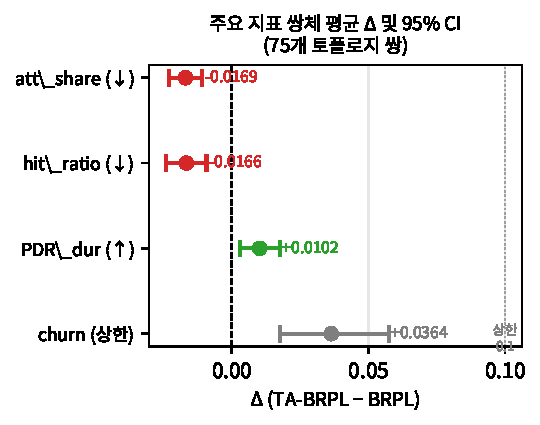
\includegraphics[width=\columnwidth]{fig_jkcs_delta_ci.pdf}
\caption{주요 지표 쌍체 평균 $\Delta$ 및 95\% CI (75개 토폴로지 쌍).
  att\_share/hit\_ratio: H1 채택(0 왼쪽);
  PDR\_dur: H2 채택(0 오른쪽);
  churn: H3 CI 상한 0.057 $<$ 0.1 채택.}
\label{fig:delta_ci}
\end{figure}

\subsection{밀도별 세부 결과}

\begin{table}[t]
\centering\small
\caption{밀도별 결과 (각 25쌍, Holm 보정)}
\label{tab:density}
\begin{tabular}{lrrrr}
\toprule
밀도 & $\Delta$att & 승률 & $\Delta$PDR & $p$ \\
\midrule
고밀도 & $-0.009$ & 68\%          & $+0.002$ & 0.206 \\
중밀도 & $-0.026$ & \textbf{84\%} & $+0.012$ & $<10^{-3}$ \\
저밀도 & $-0.016$ & 76\%          & $+0.016$ & $0.048$ \\
\bottomrule
\end{tabular}
\end{table}

그림~\ref{fig:box_density}는 밀도별 att\_share 분포를 보여준다.

\begin{figure}[t]
\centering
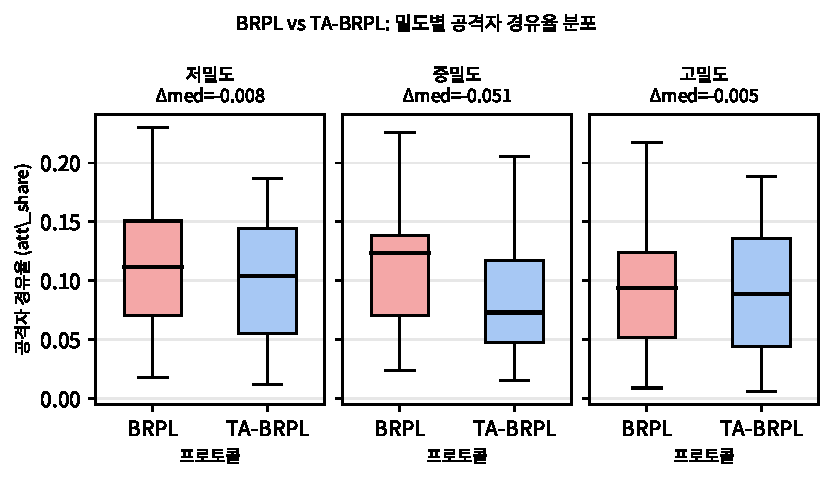
\includegraphics[width=\columnwidth]{fig_jkcs_box_density.pdf}
\caption{밀도별 BRPL vs. TA-BRPL 공격자 경유율 분포. 중밀도에서 격차가 가장 크다.}
\label{fig:box_density}
\end{figure}

\textbf{중밀도 최적.} 충분한 경로 다양성으로 신뢰 모델이 트래픽을 우회시킬 수 있되,
고밀도처럼 경로 중복성이 공격자 영향을 희석하지는 않는 구간에서 가장 강한 효과가 나타난다.

\textbf{고밀도.} 토폴로지 구조 자체가 공격자 영향을 분산시켜 한계 이득이 감소한다.

\textbf{저밀도.} 경로 선택지가 적어 우회 재구성이 자주 발생, churn 비용 +0.089.

\subsection{PDR 비열세 검증}

그림~\ref{fig:pdr_noninf}에서 전체 93.3\%의 토폴로지 쌍이 비열세 마진
($\delta = -0.02$\,pp)을 통과한다.
실패 5건은 모두 저밀도 네트워크이며, 경로 재구성 중 일시적 PDR 하락에 기인한다.
고밀도·중밀도는 전체 통과.

\begin{figure}[t]
\centering
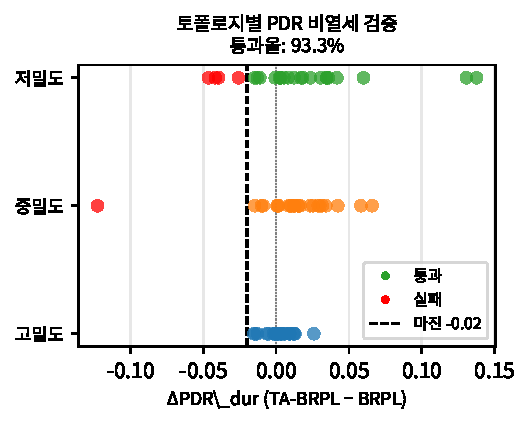
\includegraphics[width=\columnwidth]{fig_jkcs_pdr_noninf.pdf}
\caption{토폴로지별 PDR 비열세 검증 (마진 $\delta=-0.02$\,pp).
  93.3\% 통과; 실패 5건 모두 저밀도.}
\label{fig:pdr_noninf}
\end{figure}

\subsection{신뢰 성분 Ablation}

세 신호의 기여를 검증하기 위해 최소 구성 ablation을 사전 수행했다
(3 density $\times$ 3 topology $\times$ 1 seed, 9쌍).

\begin{table}[t]
\centering\small
\caption{최소 Ablation 결과 ($\Delta$=variant$-$BRPL, 9쌍)}
\label{tab:ablation}
\begin{tabular}{lccc}
\toprule
구성 & $\Delta$att [CI] & $\Delta$PDR & Win \\
\midrule
Full             & $-0.034$ [$-0.047$, $-0.019$] & $+0.005$ & 88.9\% \\
$T_{fwd}$ only   & $-0.007$ [$-0.026$, $+0.011$] & $-0.034$ & 55.6\% \\
$T_{fwd}{+}T_{ctrl}$ & $-0.008$ [$-0.027$, $+0.011$] & $-0.030$ & 55.6\% \\
\bottomrule
\end{tabular}
\end{table}

표~\ref{tab:ablation}에서 Full 모델만 CI가 완전히 0 아래에 위치한다.
단일/두 신호만으로는 CI가 0을 가로지르고 PDR\_dur도 하락하여,
세 신호 결합과 안정화 정책이 모두 필요함을 확인한다.

\subsection{왜 동작하는가: 결과 해석}

전체 결과를 종합하면 TA-BRPL의 이득은
``더 공격적으로 차단했기 때문''이 아니라
``더 이른 단계에서 덜 의존하게 만들었기 때문''으로 해석된다.
$T_{ctrl}$은 저-rank lure를 조기에 감지하고,
$T_{hon}$은 BRPL이 전제하는 queue advertisement의 정직성을 검증하며,
$T_{fwd}$는 실제 포워딩 불일치를 후행 증거로 제공한다.
이 세 신호가 함께 BRPL 비용에 결합되면서
공격자가 초기에는 정상처럼 행동하더라도
장기적으로는 덜 선호되는 부모로 밀려난다.

동시에 admission, dwell, switch-margin 게이트는
신뢰 하락이 곧바로 대량 parent switching으로 번지는 것을 막는다.
이 때문에 TA-BRPL은 att\_share와 hit\_ratio를 줄이면서도
churn 비용을 제한된 범위 안에 유지할 수 있었다.
특히 중밀도에서 효과가 가장 큰 것은
우회 가능한 대체 부모가 충분히 존재하면서도
토폴로지 자체가 공격자 영향을 완전히 희석하지는 않기 때문이다.


% ============================================================
\section{한계 및 위협요인}
\label{sec:discussion}

본 연구 결과는 유의미하지만, 다음 한계를 함께 고려해야 한다.

\textbf{귀책(attribution) 한계.}
$T_{fwd}$는 에코 기반 전달 신뢰를 이용하므로,
실제 드롭 위치가 상위 홉에 있을 때 그 아래의 정직한 relay가
낮은 forwarding trust를 받을 수 있다.
본 연구는 $T_{ctrl}$, $T_{hon}$, review/blacklist, dwell gate로 이를 완화했지만,
특히 저밀도 네트워크에서는 이러한 귀책 편향이 완전히 제거되지 않는다.

\textbf{정적 시뮬레이션 환경.}
실험은 Contiki-NG/Cooja와 UDGM 무선 모델에서 수행되었다.
이 설정은 재현성과 통제성 측면에서는 장점이 있으나,
실제 배치의 fading, hidden terminal, 비동기 간섭, 장기적인 링크 변화를
충분히 반영하지 못한다.
따라서 본 결과는 메커니즘 검증에는 적합하지만,
실환경 성능을 직접 대변하지는 않는다.

\textbf{공격 범위의 제한.}
본 논문은 단일 내부자 sinkhole + 50\% selective forwarding에 초점을 맞춘다.
다중 공모 공격자, version-number attack, Sybil, mobility,
온오프 공격, 공격자 간 역할 분담은 현재 범위 밖이다.
또한 RFTrust~\cite{rftrust2021}, PCC-RPL~\cite{pccrpl2022} 같은
동급 보안 라우팅과의 직접 비교도 아직 수행하지 않았다.

\textbf{파라미터 민감도.}
제시한 결과는 v13.12 파라미터 스냅샷을 기준으로 한다.
이 값들은 반복 실험을 통해 안정화된 조합이지만,
밀도와 공격 강도에 따라 최적점이 달라질 수 있다.
특히 sparse 네트워크에서 churn 비용이 더 크게 나타난 것은,
공통 파라미터가 모든 밀도에 동일하게 최적인 것은 아님을 시사한다.

\textbf{에너지/지연 비용 미측정.}
본 논문은 att\_share, hit\_ratio, PDR, churn을 주 지표로 삼았고,
제어 메시지 증가량, CPU/메모리 부담, 에너지 소모, per-packet latency는
정량적으로 보고하지 않았다.
실배치 가능성을 논하려면 향후 이 비용 축이 반드시 보완되어야 한다.


% ============================================================
\section{결론}
\label{sec:conclusion}

본 논문은 sinkhole 공격을 경로 장악 → 가용성 파괴의 2단계 위협으로 정의하고,
방어 1차 목표를 PDR이 아닌 \emph{경로 장악 억제}로 재설정한 \textbf{TA-BRPL}을 제안했다.

실험 결과, TA-BRPL은 att\_share와 hit\_ratio를 유의하게 감소시켜
공격자 의존 강도와 오염 범위를 함께 줄였다 ($p<10^{-4}$).
공격 구간 PDR은 평균적으로 개선되었고,
토폴로지의 93.3\%가 비열세 기준을 통과했다.
또한 churn 증가는 존재했지만,
95\% CI 상한이 사전 선언한 $+0.1$보다 낮아
관리 가능한 stability overhead 범위에 머물렀다.

따라서 TA-BRPL의 핵심 기여는 ``더 강한 탐지기''를 추가한 것이 아니라,
신뢰를 BRPL 부모 선택 metric에 직접 결합하면서도
admission, dwell, switch-margin으로 라우팅 진동을 제어하는
\emph{안정화된 trust-aware routing} 설계를 제시한 데 있다.
이는 LLN 보안에서 route capture 억제와 routing stability가
별개의 문제가 아니라 하나의 공동 설계 문제임을 보여준다.

\subsection*{향후 연구}

후속 연구는 다음 네 방향으로 확장될 수 있다.

\textbf{다중 공격자 및 공모 시나리오.}
본 실험은 단일 내부자 공격자를 가정했다.
두 개 이상의 공격자가 공모해 서로의 신뢰 신호를 보강하거나,
역할을 분담해 탐지를 회피하는 시나리오에서
TA-BRPL의 방어 효과가 어떻게 달라지는지 검증이 필요하다.
특히 공격자 간 공모가 $T_{ctrl}$의 rank 이상 탐지를 희석시킬 수 있는지가 핵심 쟁점이다.

\textbf{현실적 손실 환경 및 이동성.}
UDGM은 결정론적 거리 기반 전송 모델로,
실제 배치의 fading, shadowing, hidden terminal, 비동기 간섭을 충분히 재현하지 못한다.
Unit Disk Graph 모델을 넘어 TOSSIM, MiXiM 또는 실측 trace 기반 채널 모델로 확장하고,
노드 이동성이 있는 환경에서 $T_{fwd}$ 귀책 정확도와 churn 비용을 재평가할 계획이다.

\textbf{온오프 및 전략적 공격자.}
공격자가 신뢰 측정 주기에 맞춰 정상 행동과 드롭을 교번하는 온오프 공격은
EWMA 기반 신뢰 감쇠를 의도적으로 우회할 수 있다.
비대칭 EWMA($\lambda_d < \lambda_u$) 파라미터 조정과
관측 창 기반 review/blacklist의 내성을 체계적으로 분석할 필요가 있다.

\textbf{에너지·지연 오버헤드 및 동급 비교.}
현재 평가는 att\_share, hit\_ratio, PDR, churn에 집중하며
제어 메시지 증가량, 에너지 소모, per-packet latency를 정량화하지 않았다.
실배치 가능성을 평가하려면 이 비용 축이 보완되어야 한다.
또한 RFTrust~\cite{rftrust2021}, PCC-RPL~\cite{pccrpl2022} 같은
동급 신뢰 기반 라우팅과의 직접 비교를 통해
TA-BRPL의 상대적 강점과 적용 범위를 더 엄밀히 규명할 필요가 있다.


% ============================================================
\bibliography{references}

\end{document}
